\documentclass[boxes, qed]{homework}
\usepackage{xcolor,amsmath,listings}
\usepackage{graphicx}
\usepackage[backend=biber, style=mla, citestyle=authoryear]{biblatex}

\addbibresource{homework-9.bib}
\graphicspath{ {./images/} }

\name{Rohit Wason}
\course{Math 560}
\term{Spring 2021}
\hwnum{(\#10, Regression)}

\newcommand{\bigzero}{\mbox{\normalfont\Large\bfseries 0}}
\newcommand{\rvline}{\hspace*{-\arraycolsep}\vline\hspace*{-\arraycolsep}}

\begin{document}

\begin{problem}Given:\\
  $n=500$\\
  Mean height of the fathers, $\bar{x}=67.9$ (explanatory vaiable)\\
  Standard deviation of the height of fathers, $s_x=2.75$\\
  Mean height of the sons, $\bar{y}=68.7$ (response vaiable)\\
  Standard deviation of the height of sons, $s_y=2.83$\\
  The correlation between the heights of the sons and their fathers, $r=0.5$.
\end{problem}
\begin{solution}
  (a) Give a $99$\% prediction interval for the height of a son whose father is $70$ inches tall.\\
  Using $b_1=r(s_y/s_x)$ and $b_0=\bar{y}-b_1\bar{x}$ we have that
  $$b_1=0.5(2.83/2.75)\approx 0.5145$$
  $$b_0=68.7 - 0.5145(67.9) \approx 33.7654$$
\end{solution}

\begin{problem}
  \begin{tabular}{l|l}\hline
    Year($x$) & Kilobits($y$)\\\hline
    1971&1\\\hline
    1980&62.5\\\hline
    1987&1000\\\hline
    1993&16000\\\hline
    1998&125000\\\hline
    2000&250000\\\hline
    2002&500000\\\hline
    2004&976562.5\\\hline
  \end{tabular}
\end{problem}
\begin{solution}
  We build the model
  \begin{lstlisting}[backgroundcolor = \color{lightgray},language = R]
    lmKilo=lm(Kilobits~Year, data = dram)
    lmKilo$coefficients
    > (Intercept)      Year 
    > -40886934.88     20644.12
  \end{lstlisting}
  to receive the coefficients $b_0=-40886934.88, b_1=20644.12$.
  Therefore the equation of the least-square regression line is
  $$\hat{y}=-40886934.88 + 20644.12(x)$$

  $s_x=11.6795$\\
  $s_y=347560.1$\\
  Using $b_1=r(s_y/s_x)$ and $b_0=\bar{y}-b_1\bar{x}$ we have that
\end{solution}
\pagebreak

\section*{Project details}
\subsection*{Introduction}
According to the World Health Organization (WHO) stroke is the 2nd leading cause of death globally, 
responsible for approximately 11\% of total deaths. This dataset is used to predict whether a patient
is likely to get stroke based on the input parameters like gender, age, various diseases, and smoking 
status. We can use this dataset to state hypotheses of correlation between various explanatory
variables (like, age, bmi, marital status, residence type, etc.) and the result that they have had
a stroke.\\
The dataset used here can be found on Kaggle, a public competetion forum
where data scientists and novices collaborate to find answers in complex datasets
(\cite{kaggle}). This dataset contains $5110$ data points with $12$ variables:
\begin{enumerate}
  \item \textbf{id:} unique identifier
  \item \textbf{gender:} "Male", "Female" or "Other"
  \item \textbf{age:} age of the patient
  \item \textbf{hypertension:} 0 if the patient doesn't have hypertension, 1 if the patient has hypertension
  \item \textbf{heart\_disease:} 0 if the patient doesn't have any heart diseases, 1 if the patient has a heart disease
  \item \textbf{ever\_married:} ``No'' or ``Yes''
  \item \textbf{work\_type:} ``children'', ``Govt\_jov'', ``Never\_worked'', ``Private'' or ``Self-employed''
  \item \textbf{Residence\_type:} "Rural" or "Urban"
  \item \textbf{avg\_glucose\_level:} average glucose level in blood
  \item \textbf{bmi:} body mass index
  \item \textbf{smoking\_status:} "formerly smoked", "never smoked", "smokes" or "Unknown"*
  \item \textbf{stroke:} 1 if the patient had a stroke or 0 if not
\end{enumerate}

\subsection*{Methods}
According to stroke.org, a non-profit organization dedicated to public awareness about,
and prevention of common causes of stroke, smoking, lack of physical activity, diabetes and 
obesity are leading factors that could lead to stroke (\cite{strokeorg}).\\
In particular the following questions are of interest:
\begin{enumerate}
  \item \textbf{Is there a strong correlation between stroke and other conditions, 
  like heart disease, or hypertension?}\\
  A histogram of whether heart-disease is present in a data point:\\
  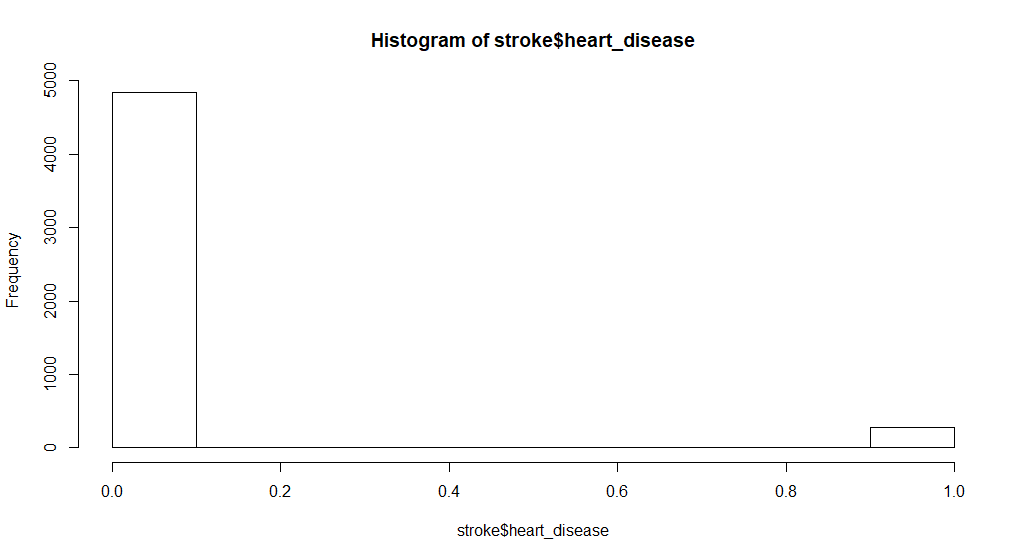
\includegraphics[scale=.5]{stroke-heart}

  \item \textbf{Does BMI indicate the occurence of stroke?}\\
  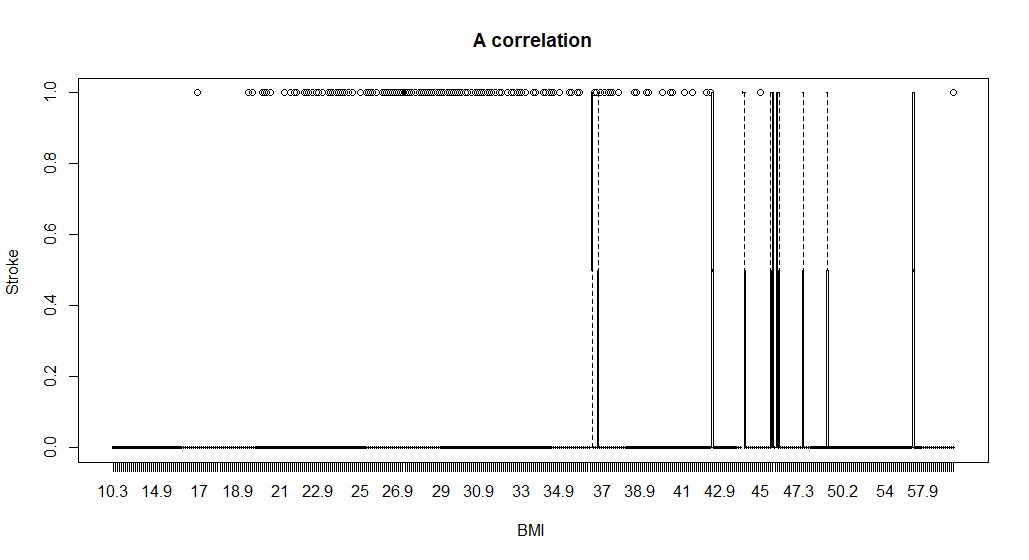
\includegraphics[scale=.5]{stroke-bmi}
\end{enumerate}

\pagebreak
\printbibliography

\end{document}
